Dans cette partie concernant l'implémentation, nous allons présenter les différentes technologies, méthodes et composants utilisés afin de mener à bien le développement de notre application. Des captures d'écran illustreront le résultat final.

% TODO: screen des fichiers
\subsection{Structure du projet et arborescence des fichiers}

\subsection{APIs}
Pour échanger les informations requises, notre application interagit avec des \acrshort{api}s externes permettant d'obtenir et persister les données nécessaires aux différentes fonctionnalités proposées, comme illustré à la figure \ref{apis_usage}.
\begin{figure}
    \begin{center}
        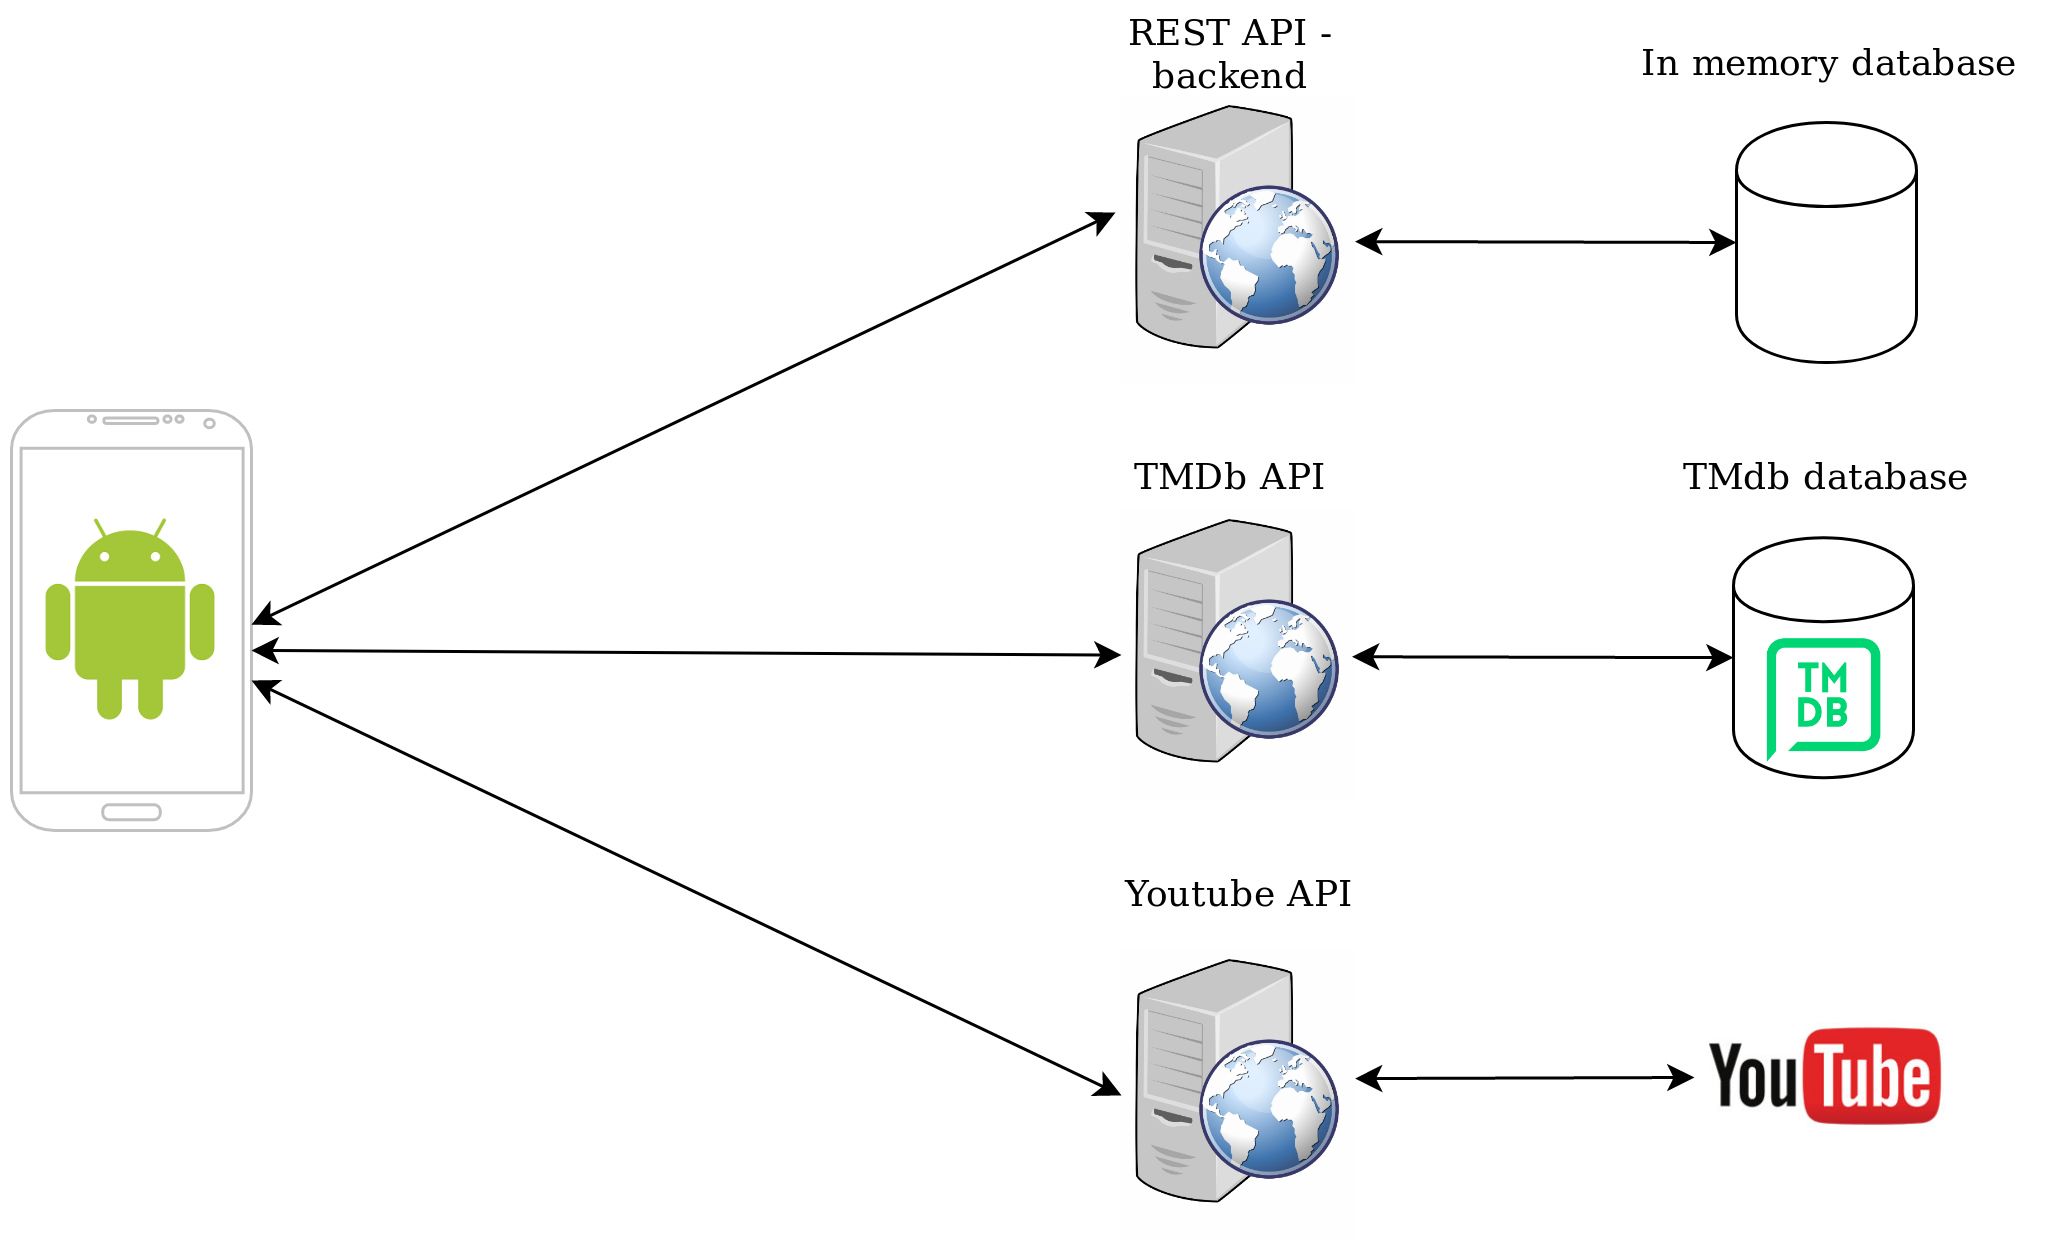
\includegraphics[width=0.8\textwidth]{img/schemas/APIs.png}
    \end{center}
    \caption{Usage des APIs}
    \label{apis_usage}
\end{figure}

\subsubsection{API TMDb}
L'\acrshort{api} principalement utilisée dans notre projet est celle proposée par \textit{The Movie Database} (TMDb) \cite{tmdb} qui offre toutes les informations sur les films et les acteurs. Nous avons également considéré \textit{The Open Movie Database} \cite{omdb}, mais elle offre beaucoup moins de possibilités. Nous interagissons avec cette \acrshort{api} en envoyant des requêtes HTTP en fonctions des besoins, nous recevons en retour les informations au format \acrshort{json}. La route GET : \mintinline{text}{/discover/movie} nous retournera les informations visibles au listing \ref{tmdb_example} au format \acrshort{json}.
\bigbreak
\begin{code}
    \begin{minted}[bgcolor=mygray,breaklines,breaksymbol=,linenos,frame=single,stepnumber=1,tabsize=2]{json}
{
  "page": 1,
  "total_results": 10000,
  "total_pages": 500,
  "results": [
    {
      "popularity": 533.832,
      "vote_count": 1707,
      "video": false,
      "poster_path": "/db32LaOibwEliAmSL2jjDF6oDdj.jpg",
      "id": 181812,
      "adult": false,
      "backdrop_path": "/jOzrELAzFxtMx2I4uDGHOotdfsS.jpg",
      "original_language": "en",
      "original_title": "Star Wars: The Rise of Skywalker",
      "genre_ids": [ 28, 12, 878 ],
      "title": "Star Wars: The Rise of Skywalker",
      "vote_average": 6.7,
      "overview": "The surviving Resistance faces the First Order ...",
      "release_date": "2019-12-18"
    },
    ...
  ]
    \end{minted}
    \caption{Exemple de données retournées par TMDb}
    \label{tmdb_example}
\end{code}
\bigbreak

\subsubsection{API REST Backend}
Certaines données de l'application nécessitent d'être persistées, c'est pourquoi nous avons choisi de mettre en place un backend basé sur Akka HTTP \cite{akka} en Scala. Le Scala est un langage relativement proche du Kotlin qui fait également usage de la \acrshort{jvm} et offre de nombreux atouts comme un typage fort, abstraction et programmation orientée objet. Tout cela avec une syntaxe permettant d'écrire le code de manière simple, concise et déclarative. Pour toutes ces raisons, le choix de ce langage nous semblait judicieux. Les routes mises à disposition par cette API REST nous permettent de persister les informations telles que les comptes des utilisateurs, les relations d'abonnements entre eux et les appréciations des films. Elles permettent également de s'authentifier, s'enregistrer et rechercher un utilisateur.

\subsubsection{API YouTube}
Pour chaque film, TMDb nous offre une liste de vidéos YouTube, comprenant des \textit{trailers} et \textit{teasers} du film. Nous avons alors fait usage de l'\acrshort{api} officielle YouTube \cite{youtube} pour intégrer ces vidéos. Il faut obligatoirement créer une clé \acrshort{api} dans son compte Google pour pouvoir utiliser cette \acrshort{api}. On peut utiliser cette \acrshort{api} globalement de deux manières différentes sur Android :
\begin{itemize}
    \item \mintinline{text}{YouTubePlayerView} et \mintinline{text}{YouTubePlayerFragment} : offrent un plus grand contrôle sur la gestion de l'interface et des contrôles d'une vidéo ainsi que de son cycle de vie au prix de plus de code à écrire et à gérer.
    \item \mintinline{text}{YouTubeStandalonePlayer}: la manière plus simple et rapide d'utiliser l'\acrshort{api}, utilise l'application officielle YouTube. Le player attend l'identifiant d'une vidéo et la clé \acrshort{api} et démarre l'activité de l'application officielle YouTube.
\end{itemize}

Nous avons décidé d'utiliser la deuxième méthode car nous n'avons pas besoin d'un contrôle fin sur le lancement des vidéos. Pour chaque vidéo obtenue sur la vue des détails d'un film, nous commençons par récupérer un \textit{thumbnail} de chaque vidéo avec ce lien : \mintinline{text}{https://img.youtube.com/vi/$youtubeId/1.jpg}. Nous superposons ensuite une icône "play" et ajoutons un listener qui démarre la vidéo sur chaque \textit{thumbnail}. Un \mintinline{kotlin}{catch} de \mintinline{kotlin}{ActivityNotFoundException} est inclu avec affichage d'un message dans un "toast" dans le cas où l'utilisateur n'a pas l'application officielle YouTube installée sur son appareil.

\subsection{Fragments}
Toutes les vues de l'application sont implémentées à l'aide de fragments. Chaque fragment est associé à un layout (fichier \acrshort{xml}) qui décrit son aspect graphique. Le code Kotlin propre au fragment nous permet uniquement de définir une implémentation qui permet l'interaction entre les différents composants graphiques de la vue et la logique métier de l'application. Notre code est ainsi réutilisable dans plusieurs vues différentes.

\subsection{Single Activity}
Selon le cours et la documentation officielle d'Android \cite{docandroid}, l'architecture actuellement conseillée pour le développement d'une application repose sur le principe de n'utiliser qu'une seule activité composée de fragments, représentant les vues de l'application, illustré en figure \ref{single_activity}.
\begin{figure}
    \begin{center}
        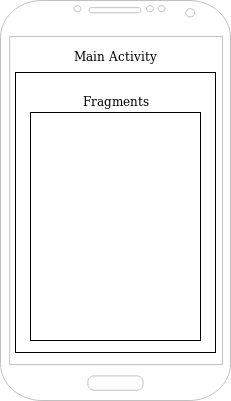
\includegraphics[width=0.5\textwidth]{img/schemas/Single_Activity.png}
    \end{center}
    \caption{Représentation d'une unique activité Android}
    \label{single_activity}
\end{figure}

\subsection{Navigation component}
Plusieurs possibilités s'offraient à nous concernant la navigation entre les différents fragments. Nous avons choisi d'expérimenter la nouvelle méthode proposée par la documentation officielle d'Android \cite{docandroid} qui est très intéressante et efficace.
Cette méthode repose sur un graphe de navigation qui est éditable graphiquement ou en \acrshort{xml}, comme illustré à la figure \ref{nav_graph}. Les noeuds de ce graphe sont les relations entre les différents fragments de l'application et les arcs symbolisent les actions de navigation d'un fragment à un autre avec des éventuelles données passées en arguments de ces actions. Ce composant de navigation génère ainsi le code des actions de navigation en fonction de ce qui a été décrit en \acrshort{xml}.
\begin{figure}
    \begin{center}
        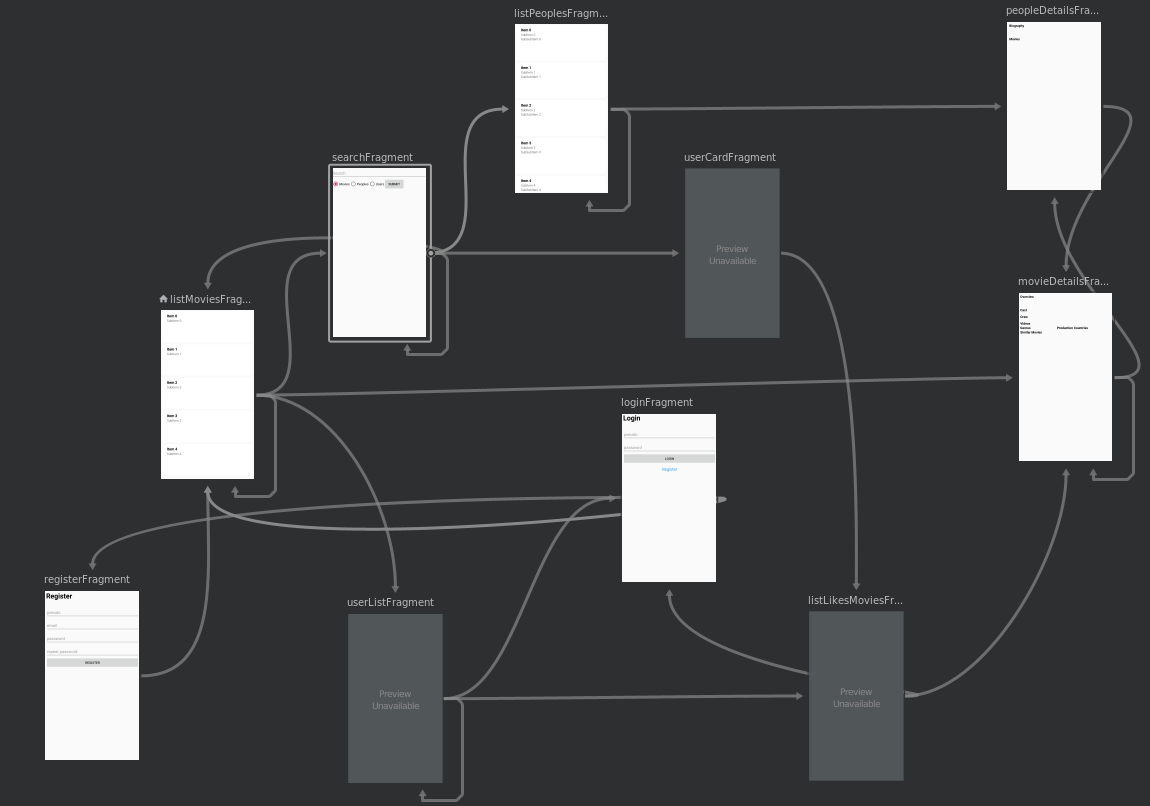
\includegraphics[width=1\textwidth]{img/screenshots/nav_graph.png}
    \end{center}
    \caption{Graphe de navigation de notre application}
    \label{nav_graph}
\end{figure}

Un exemple de code qui permet de naviguer de la liste des films vers les détails d'un film en utilisant cette classe générée automatiquement est disponible au listing de code \ref{nav_kotlin}.
\bigbreak
\begin{code}
    \begin{minted}[bgcolor=mygray,breaklines,breaksymbol=,linenos,frame=single,stepnumber=1,tabsize=2]{kotlin}
view.findNavController()
    .navigate(ListMoviesFragmentDirections
        .actionListMoviesFragmentToMovieDetailsFragment(item.id, item.urlImg))
    \end{minted}
    \caption{Exemple de navigation}
    \label{nav_kotlin}
\end{code}
\bigbreak


\subsubsection{Arguments}
Il est également possible de définir des arguments transmissibles entre les différents fragments, la classe générée automatiquement prendra en compte ces derniers. Du côté du fragment qui sera appelé, une méthode très pratique est à disposition, permettant de réceptionner ces arguments, comme décrit dans le listing \ref{args_kotlin}.
\bigbreak
\begin{code}
    \begin{minted}[bgcolor=mygray,breaklines,breaksymbol=,linenos,frame=single,stepnumber=1,tabsize=2]{kotlin}
private val args: MovieDetailsFragmentArgs by navArgs()
movieId = args.id
urlImg = args.urlImg
    \end{minted}
    \caption{Arguments du graphe de navigation en Kotlin}
    \label{args_kotlin}
\end{code}
\bigbreak


\subsection{Volley}
\subsubsection{Généralités}
Notre application est majoritairement composée d'appels HTTP à diverses \acrshort{api}s. Nous avons utilisé la librairie Android conseillée dans la documentation officielle \cite{docandroid}, Volley \cite{volley}. Elle supporte nativement les requêtes sur des chaines de caractères bruts, des images ou du \acrshort{json}. Le listing \ref{volley_kotlin_simple} décrit un exemple d'utilisation : tout d'abord il faut instancier une queue de requêtes, ensuite définir deux \textit{callbacks} traitant les cas de réussite ou d'échec de la requête, enfin ajouter ces \textit{callbacks} à la queue de requêtes. Volley exécute ensuite les requêtes se trouvant dans la queue de manière asynchrone (sans bloquer le \textit{thread} principal d'affichage) et transparente pour l'utilisateur. Il est conseillé de déclarer une seule instance de Volley avec le \textit{pattern} singleton.
\bigbreak
\begin{code}
    \begin{minted}[bgcolor=mygray,breaklines,breaksymbol=,linenos,frame=single,stepnumber=1,tabsize=2]{kotlin}
val textView = findViewById<TextView>(R.id.text)
val queue = Volley.newRequestQueue(this)
val url = "http://www.google.com"
val stringRequest = StringRequest(Request.Method.GET, url,
        Response.Listener<String> { response ->
            textView.text = "Response is: ${response.toString()}"
        },
        Response.ErrorListener { textView.text = "That didn't work!" })
queue.add(stringRequest)
    \end{minted}
    \caption{Usage de la librairie Volley}
    \label{volley_kotlin_simple}
\end{code}
\bigbreak

\subsubsection{Asynchronisme}
Dans la majorité des cas, la logique de l'application requiert d'avoir reçu certaines informations en provenance des APIs avant de pouvoir les afficher sur la vue. Nous avons besoin de garantir que l'intégralité des données soient réceptionnées avant de les afficher, mais tout cela avec la contrainte de ne pas bloquer l'affichage.
Nous avons donc utilisé le mécanisme de fonctions de \textit{callback}. Le principe est simple, la fonction de \textit{callback} n'est appelée que lorsque la requête HTTP est effectué et les données réceptionnées. Un résumé de ce comportement est illustré à la figure \ref{asynchrone}.
\begin{figure}
    \begin{center}
        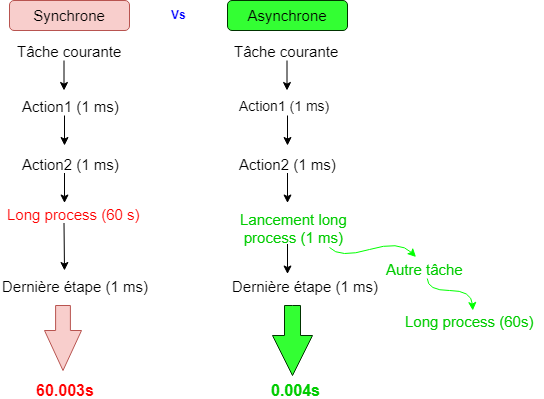
\includegraphics[width=0.8\textwidth]{img/schemas/Asynchronisme2.png}
    \end{center}
    \caption{Différences entre un fil d'exécution synchrone et asynchrone}
    \label{asynchrone}
\end{figure}

\subsubsection{Améliorations}
Etant donné le nombre d'appels HTTP important dans notre application, le code devient rapidement "pollué" par ce code long et répétitif TODO: (Steven met visible au listing 4 stp). Nous avons suivi les bonnes pratiques et simplifié cela en créant une classe \mintinline{text}{VolleyRequestController} offrant les méthodes relatives à tous les appels HTTP. Un exemple d'une requête HTTP GET utilisant cette classe est visible au listing \ref{volley_kotlin}. Nous avons également activé le cache réseau sur disque pour améliorer les performances d'affichage des vues.
\bigbreak
\begin{code}
    \begin{minted}[bgcolor=mygray,breaklines,breaksymbol=,linenos,frame=single,stepnumber=1,tabsize=2]{kotlin}
fun httpGet(URL: String, context: Context, callback: ServerCallback<JSONObject>) {
    val jsonObjReq = JsonObjectRequest(Request.Method.GET, URL, null,
    Response.Listener { response -> callback.onSuccess(response) },
    Response.ErrorListener { error ->
        Log.println(Log.DEBUG, this.javaClass.name, "error in httpGet : $error,\n$URL\n$callback")
    })
    HttpQueue.getInstance(context).addToRequestQueue(jsonObjReq)
}
    \end{minted}
    \caption{VolleyRequestController - Améliorations usage de la librairie Volley avec \textit{callback}}
    \label{volley_kotlin}
\end{code}
\bigbreak

Utilisable dans le code de la facon suivante : 

\bigbreak
\begin{code}
    \begin{minted}[bgcolor=mygray,breaklines,breaksymbol=,linenos,frame=single,stepnumber=1,tabsize=2]{kotlin}
    requestController.httpGet(url, context, object : ServerCallback<JSONObject> {
            override fun onSuccess(result: JSONObject) {
                // Traitement des données reçues dans result
            })
    }
    \end{minted}
    \caption{Usage de la librairie Volley avec \textit{callback}}
    \label{volley_kotlin}
\end{code}
\bigbreak

\subsubsection{Toolbar}
En haut de l'écran se trouve une barre comportant le nom du fragment courrant, un bouton "home" (\ref{films-tendance}) et un contrôle faisant apparaitre le menu latéral.

\subsection{Drawer}
Le drawer est un menu latéral qui apparaît de gauche à droite de l'écran. Ce menu permet d'afficher les informations relatives au profil de l'utilisateur courant. D'autre part, il propose les action de connexion, création de compte et déconnexion. Si l'utilisateur est connecté, il pourra aussi naviguer vers les vues des films aimés et du réseau d'amis.
Afin de rendre l'interface utilisateur plus conviviale, nous av
ons implémenté un \textit{drawer}, illustré à la figure \ref{drawer}. Ce \textit{drawer} repose également sur la dernière méthode proposée par la documentation d'Android \cite{docandroid}. L'interface graphique du \textit{drawer} est définie dans le \acrshort{xml} à l'aide d'un menu, et initialisée dans la \textit{main activity}. L'identifiant des différents items est nommé selon les identifiants référencés dans le graphe de navigation ce qui permet de naviguer directemnt vers le bon fragment lors de l'interaction d'un utilisateur avec ces derniers. Pour ce faire, le layout de la \textit{main activity} est de type \mintinline{text}{DrawerLayout}, elle inclut tout le contenu (\textit{top bar}, fragments de navigation, et \textit{bottom tabs}) ainsi que le \textit{drawer} qui sera affiché.
\begin{figure}
    \begin{center}
        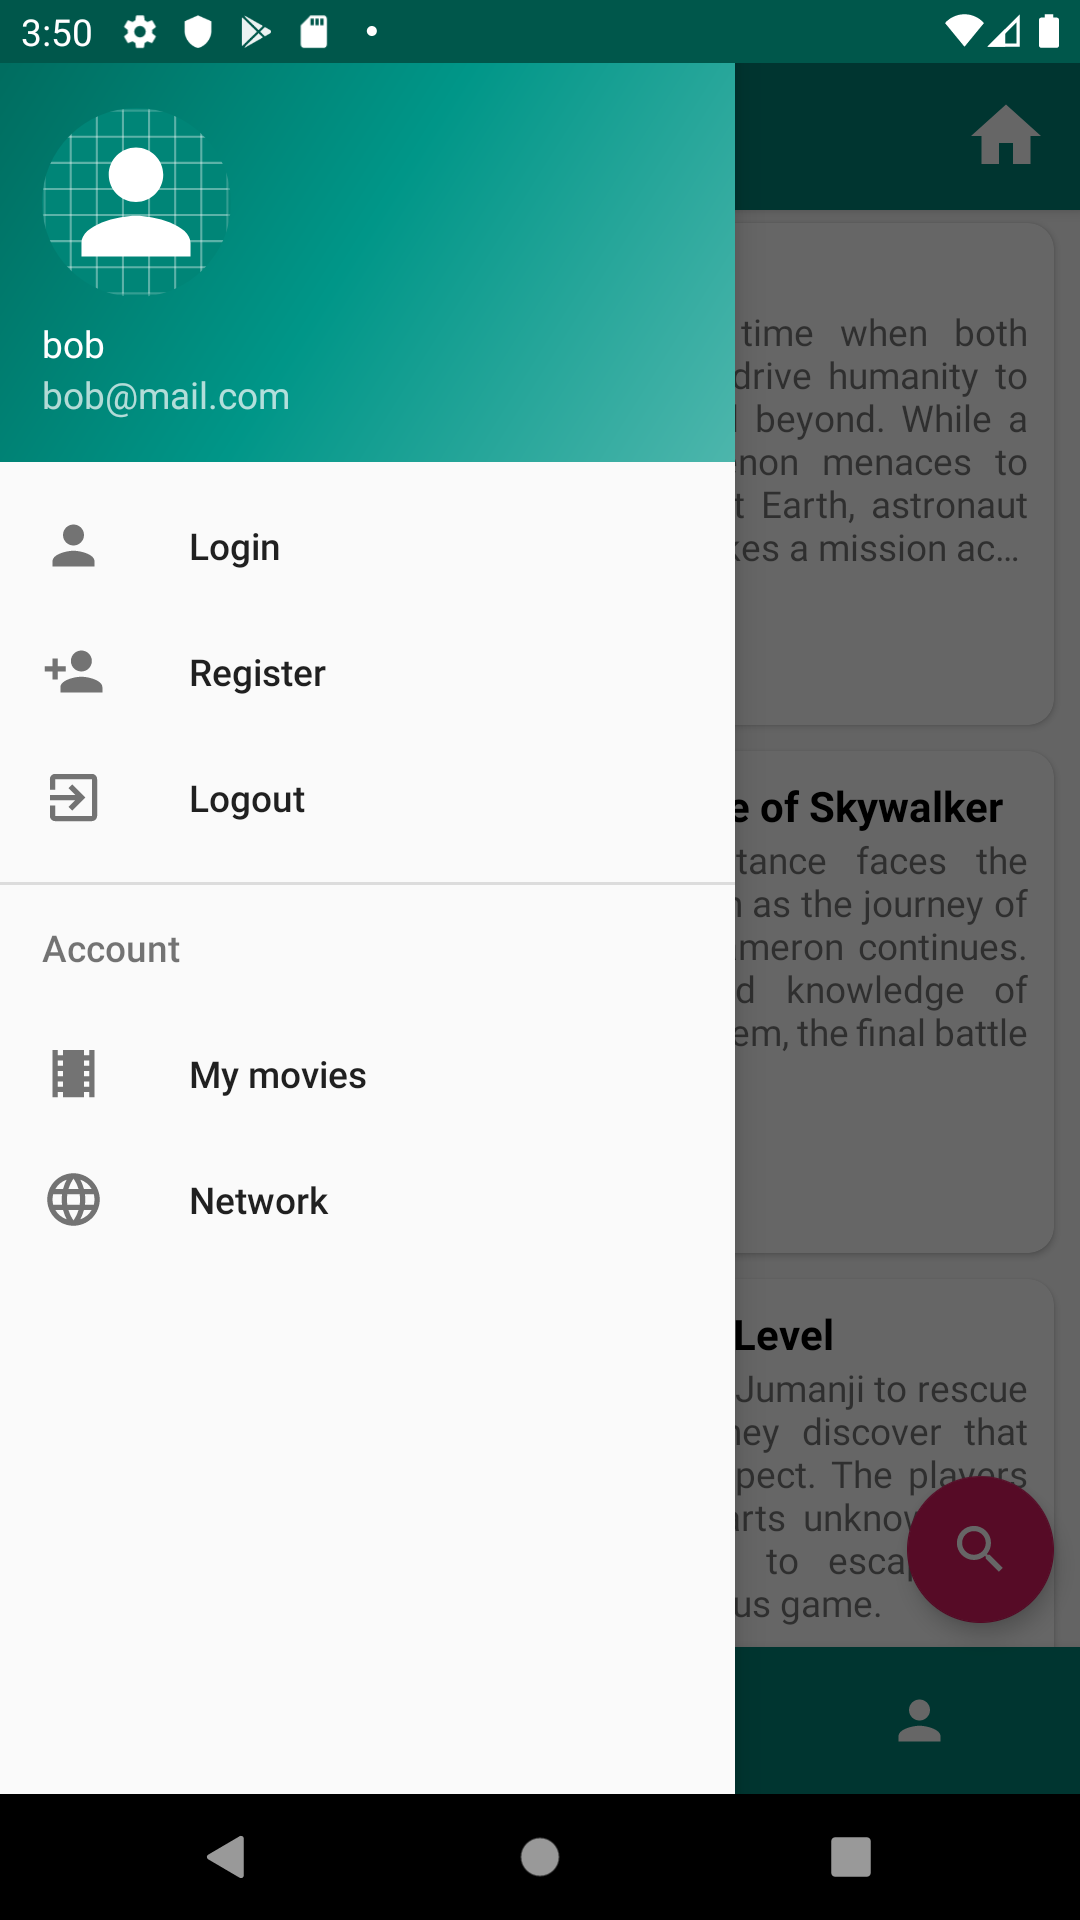
\includegraphics[width=0.5\textwidth]{img/screenshots/Drawer.png}
    \end{center}
    \caption{Drawer de l'application}
    \label{drawer}
\end{figure}

\subsection{Bottom tabs}
En bas de l'écran, des onglets de navigation sont présents, permettant de naviguer entre les vues principales de l'application, ces \textit{tabs} ont été implémentés à l'aide d'un menu classique Android défini au niveau \acrshort{xml}, illustrés à la figure \ref{tabs}. En basant l'identifiant de chaque item du menu sur les identifiants référencés dans le \textit{navigation graph}, chaque fragment est correctement appelé et affiché lors du clic sur un onglet.

\begin{figure}
    \begin{center}
        
\includegraphics[width=0.8\textwidth]{img/screenshots/Bottom_Tabs.png}
    \end{center}
    \caption{Onglets de l'application}
    \label{tabs}
\end{figure}

\subsection{View pager}

Pour les vues concernant les films appréciés/non appréciés et les utilisateurs suivis/abonnés, il était pratique de pouvoir passer d'une liste à l'autre rapidement et efficacement, comme illustré aux figures \ref{view_pager1} et \ref{view_pager2}. Nous avons donc mis en place des \textit{view pagers} qui sont en quelque sorte des sous-onglets permettant de "switcher" entre différents fragments assez rapidement. La réutilisation du code pour chaque sous-onglet (uniquement un changement de paramètre) est un avantage supplémentaire.
\begin{figure}
    \begin{center}
        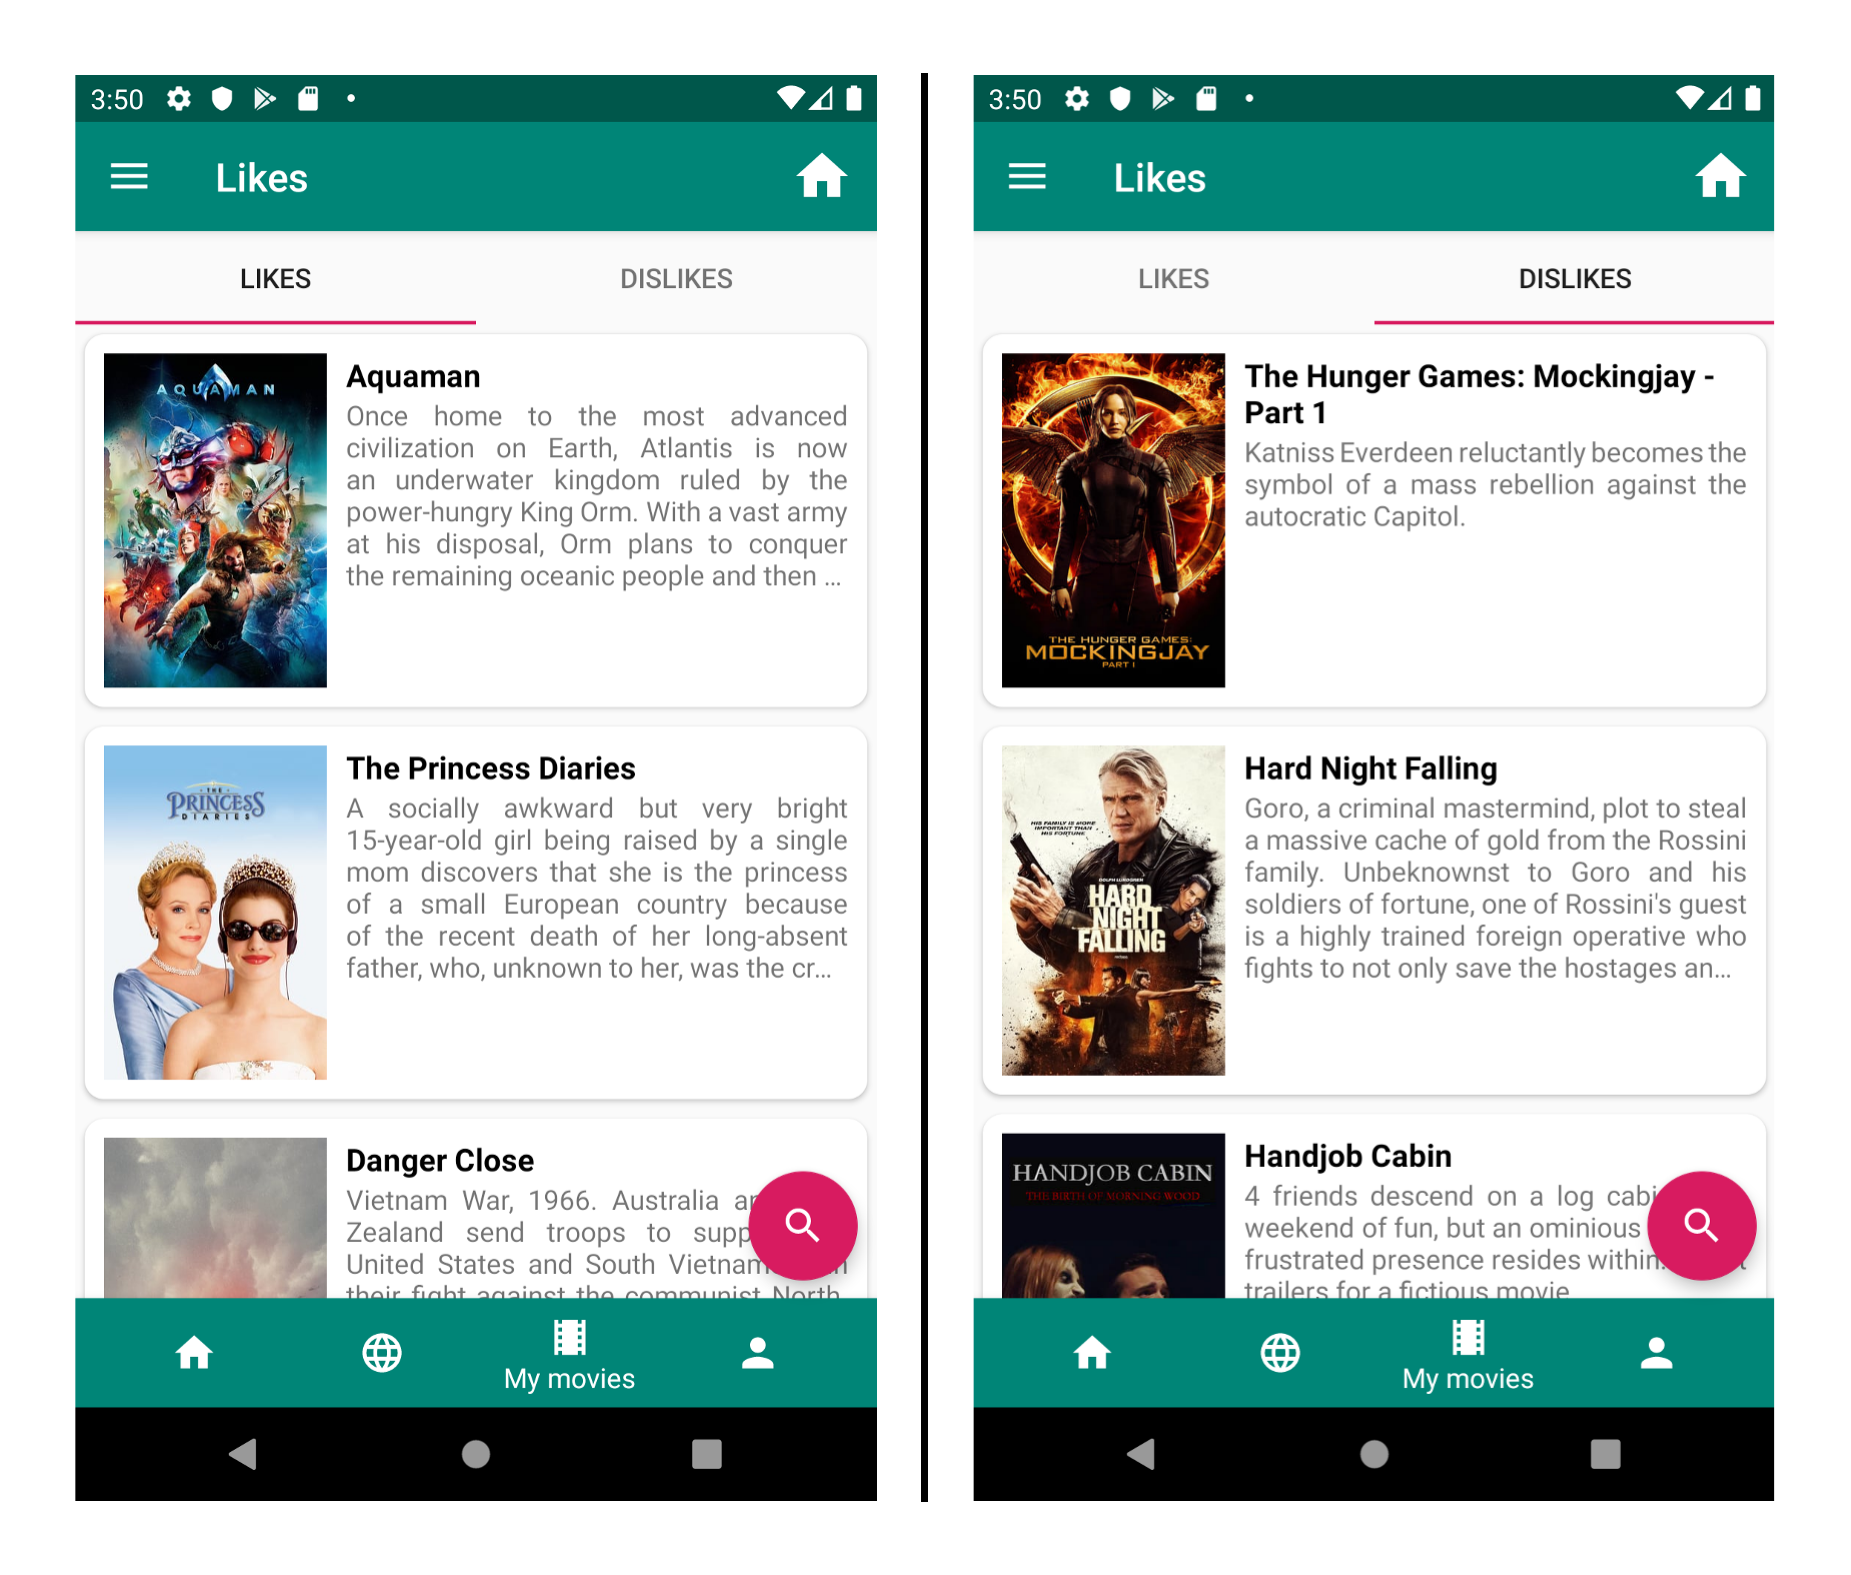
\includegraphics[width=0.8\textwidth]{img/screenshots/ViewPager1.png}
    \end{center}
    \caption{Appreciations des films dans l'application}
    \label{view_pager1}
\end{figure}

\begin{figure}
    \begin{center}
        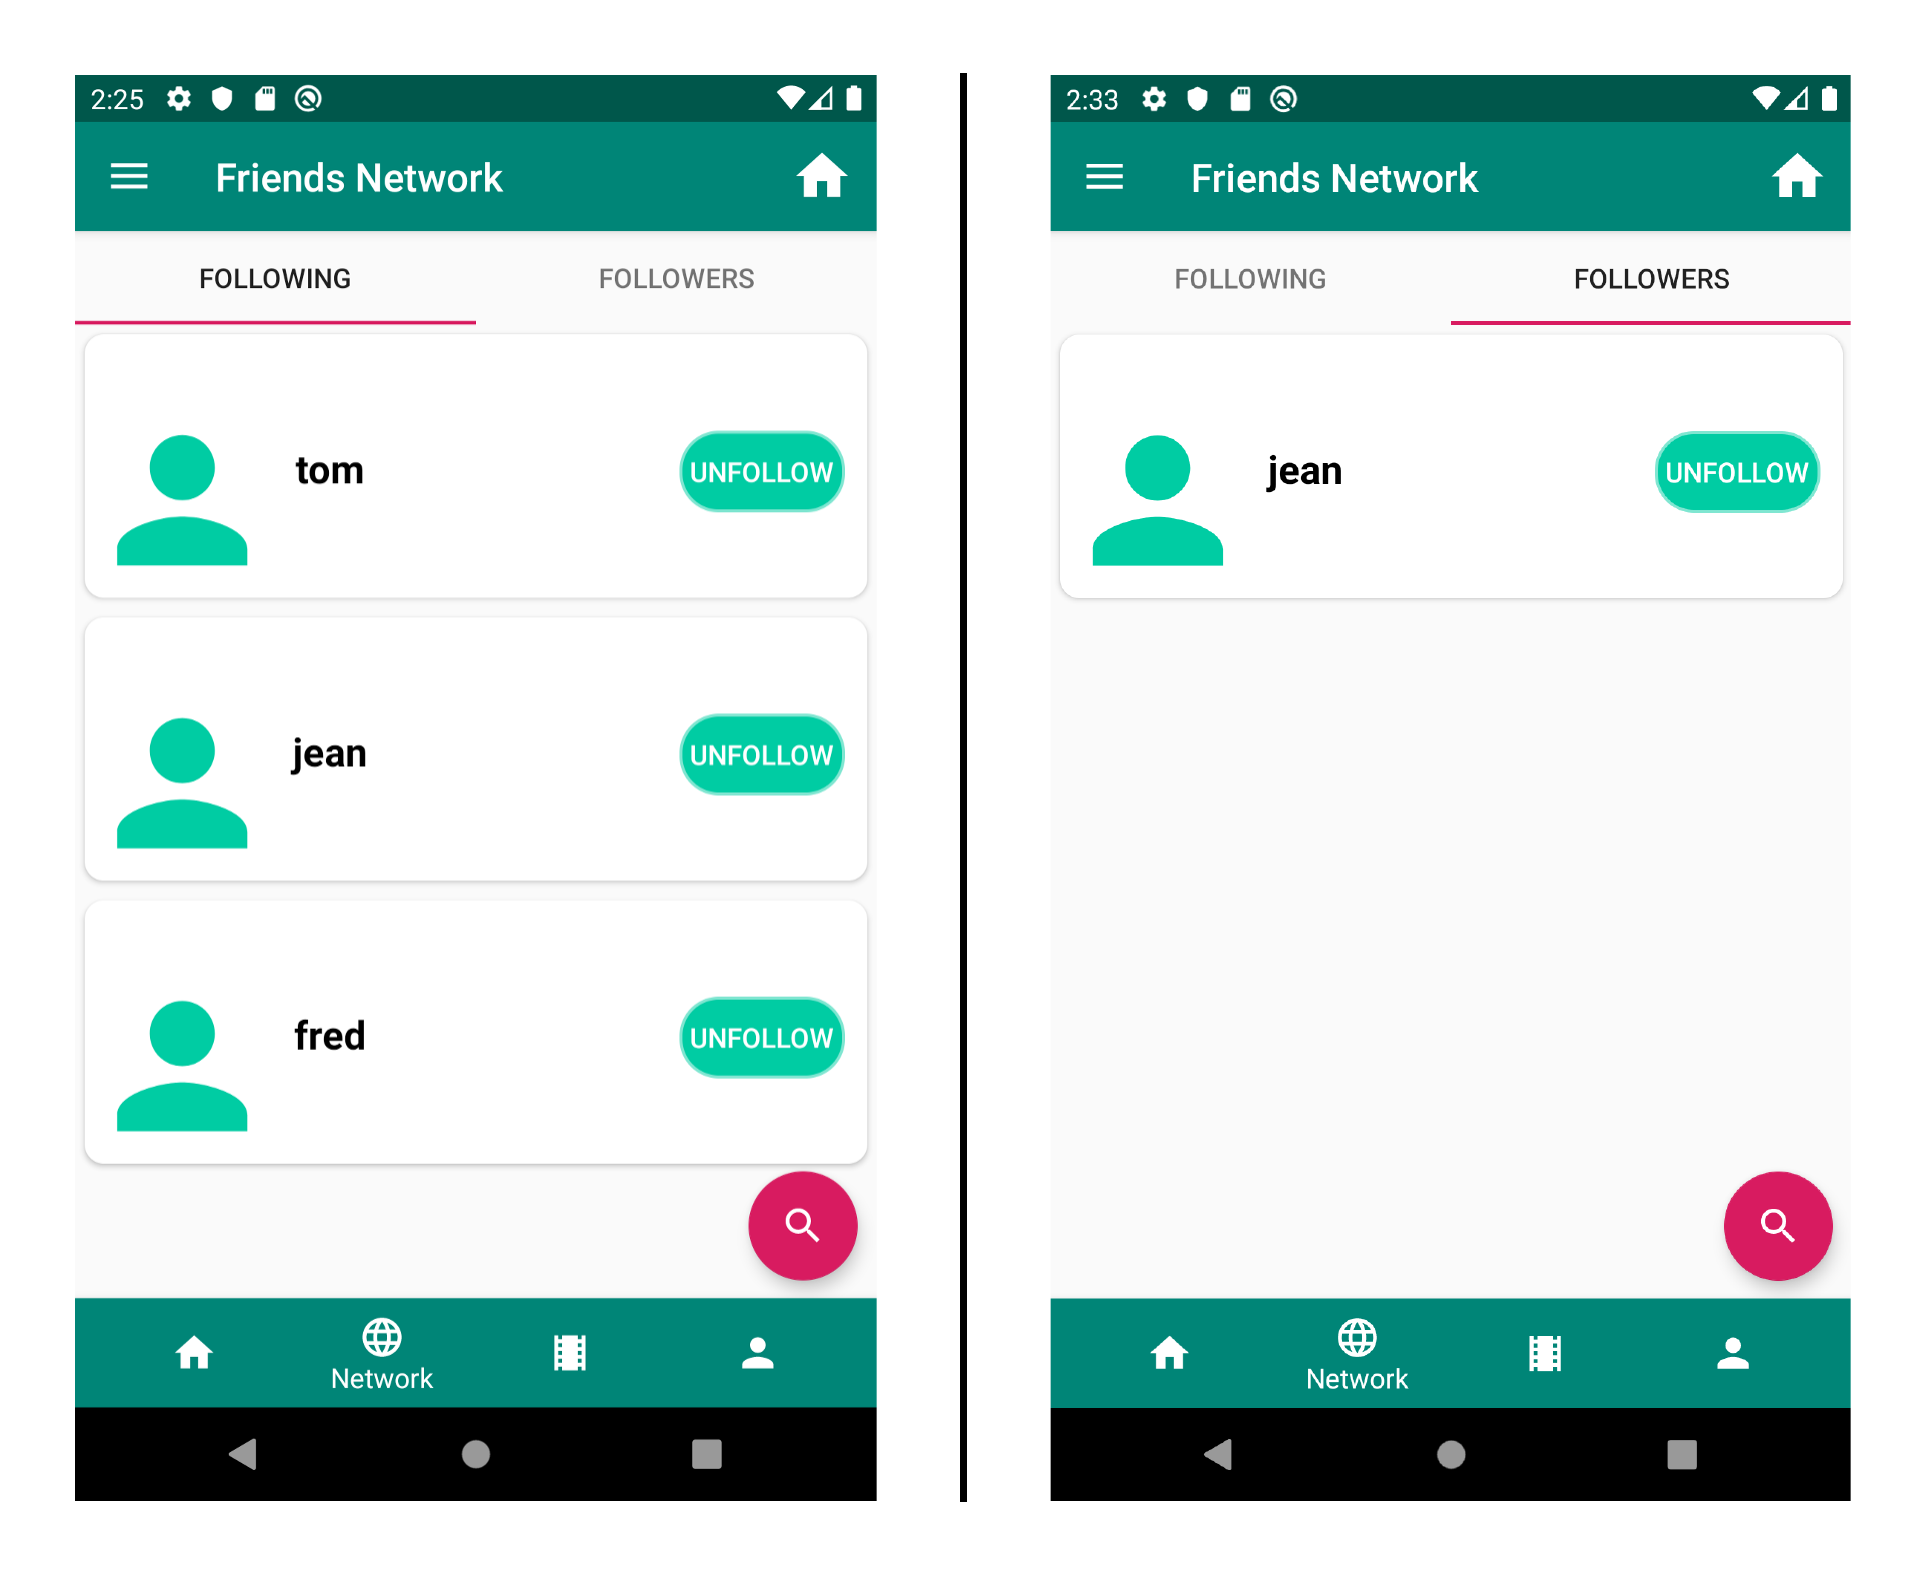
\includegraphics[width=0.8\textwidth]{img/screenshots/ViewPager2.png}
    \end{center}
    \caption{Réseau social dans l'application}
    \label{view_pager2}
\end{figure}

\subsection{Recherche}
La recherche est un fragment qui contient, au niveau \acrshort{xml}, uniquement un champ texte dans lequel les mots-clé sont saisis et un bouton radio sélectionnant dans quelle rubrique rechercher.
Lorsque l'action de recherche est effectuée, une \textit{recycler view} présentant les résutats de la recherche est affichée. La \textit{recycler view} appelée est toujours la même, nous avons uniquement le type des éléments affichés et le layout associé qui varient en fonction du type de la recherche (voir section \ref{generic-adapter}).
\begin{figure}
    \begin{center}
        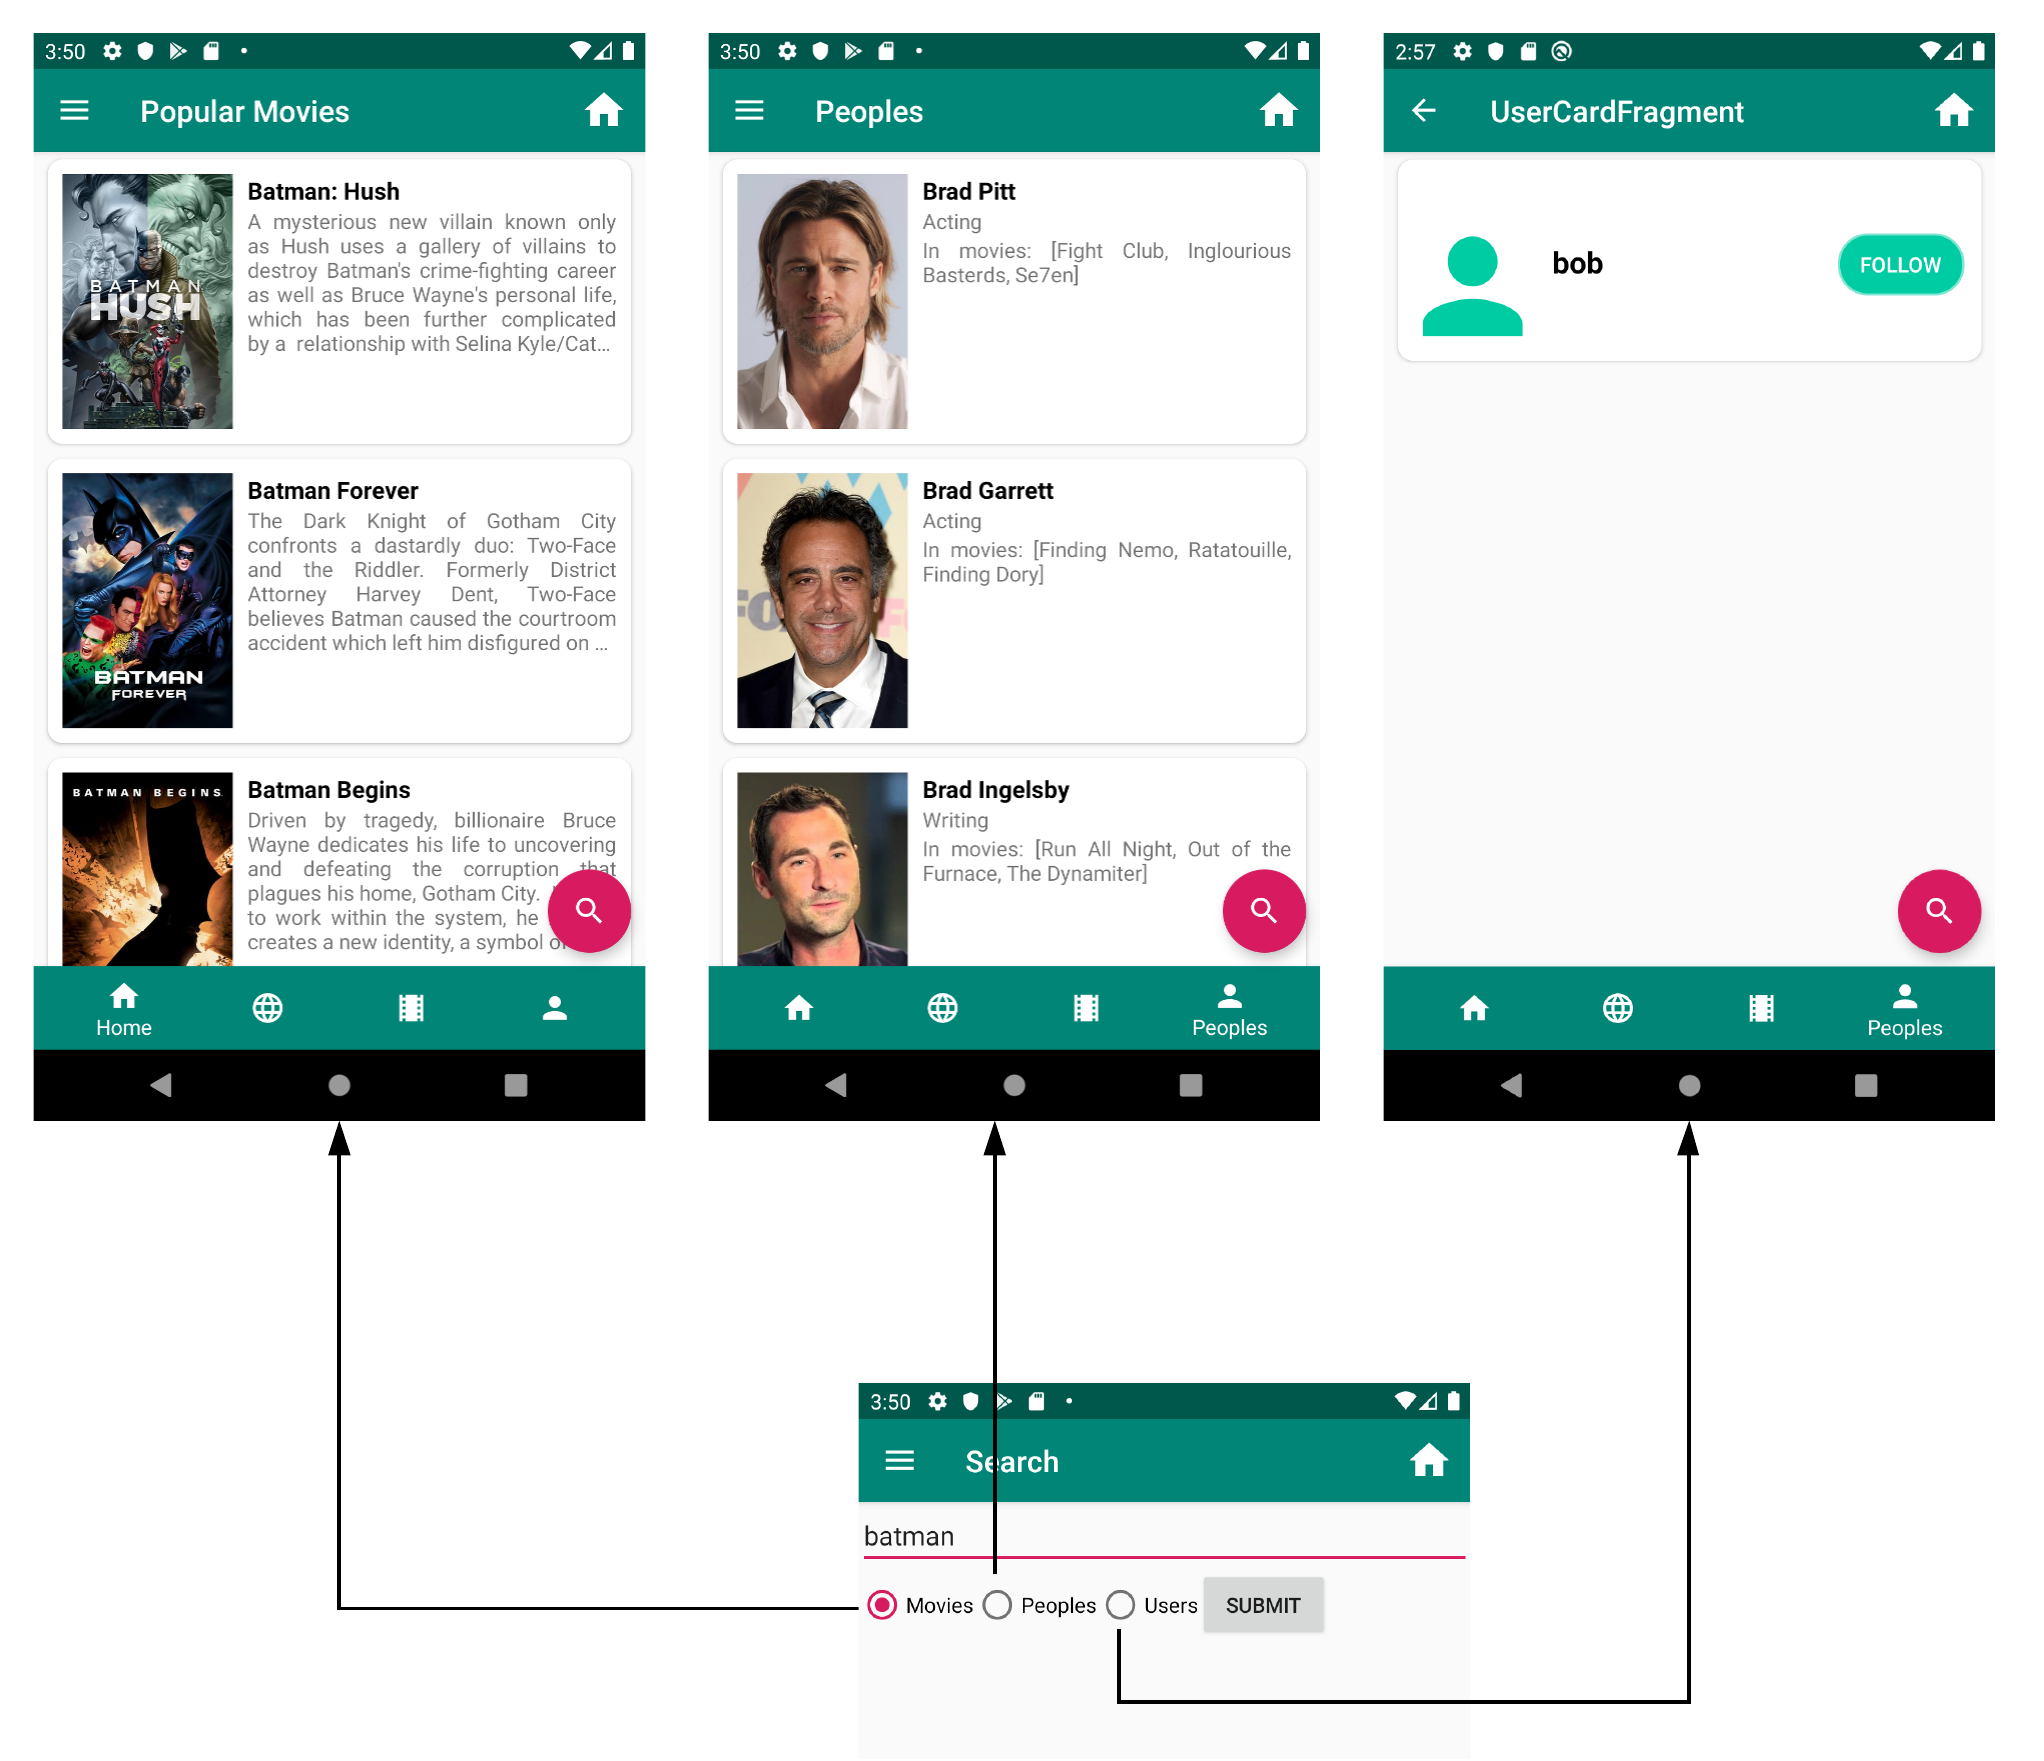
\includegraphics[width=1\textwidth]{img/schemas/Search.png}
    \end{center}
    \caption{Vue de la recherche dans l'application}
    \label{search}
\end{figure}


\subsection{Shared preferences}
Afin de stocker la session d'un utilisateur connecté à l'application, nous avons fait usage des \textit{shared preferences} qui sont un moyen simple (ensemble de clés-valeurs) et pratique de persister des information dans l'application et d'y accéder depuis les différents fragments. Deux exemples de leur utilisation sont disponibles aux listings \ref{share_prefs_kotlin1} et \ref{share_prefs_kotlin2}. Ce mécanisme permet également de vérifier qu'un utilisateur soit authentifié et de le rediriger vers la page de login dans le cas échéant.
\bigbreak
\begin{code}
    \begin{minted}[bgcolor=mygray,breaklines,breaksymbol=,linenos,frame=single,stepnumber=1,tabsize=2]{kotlin}
val sharedPref = activity?
    .getSharedPreferences(getString(R.string.preference_file_key), 
    Context.MODE_PRIVATE) ?: return
with (sharedPref!!.edit()) {
    putString(getString(R.string.pseudo), pseudo)
    putString(getString(R.string.email), email)
    putString(getString(R.string.token), token)
    commit()
}
    \end{minted}
    \caption{Création des \textit{shared preferences}}
    \label{share_prefs_kotlin1}
\end{code}
\bigbreak

\bigbreak
\begin{code}
    \begin{minted}[bgcolor=mygray,breaklines,breaksymbol=,linenos,frame=single,stepnumber=1,tabsize=2]{kotlin}
val auth = Common.getAuth((activity as MainActivity).
    getSharedPreferences(getString(R.string.preference_file_key),
    Context.MODE_PRIVATE), view.context)
if (auth != null) {
    ....
}
    \end{minted}
    \caption{Vérification des \textit{shared preferences}}
    \label{share_prefs_kotlin2}
\end{code}
\bigbreak

\subsection{FAB}
Un \textit{floating action button} (FAB) est disponible en bas à droite de l'écran, comme illustré dans la figure \ref{fab} un écouteur sur ce bouton est défini dans la \textit{main activity} permettant d'intercepter les interactions des utilisateurs. Lorsqu'une interaction est détectée, une redirection vers le fragment dédié à la recherche est effectuée.
\begin{figure}
    \begin{center}
        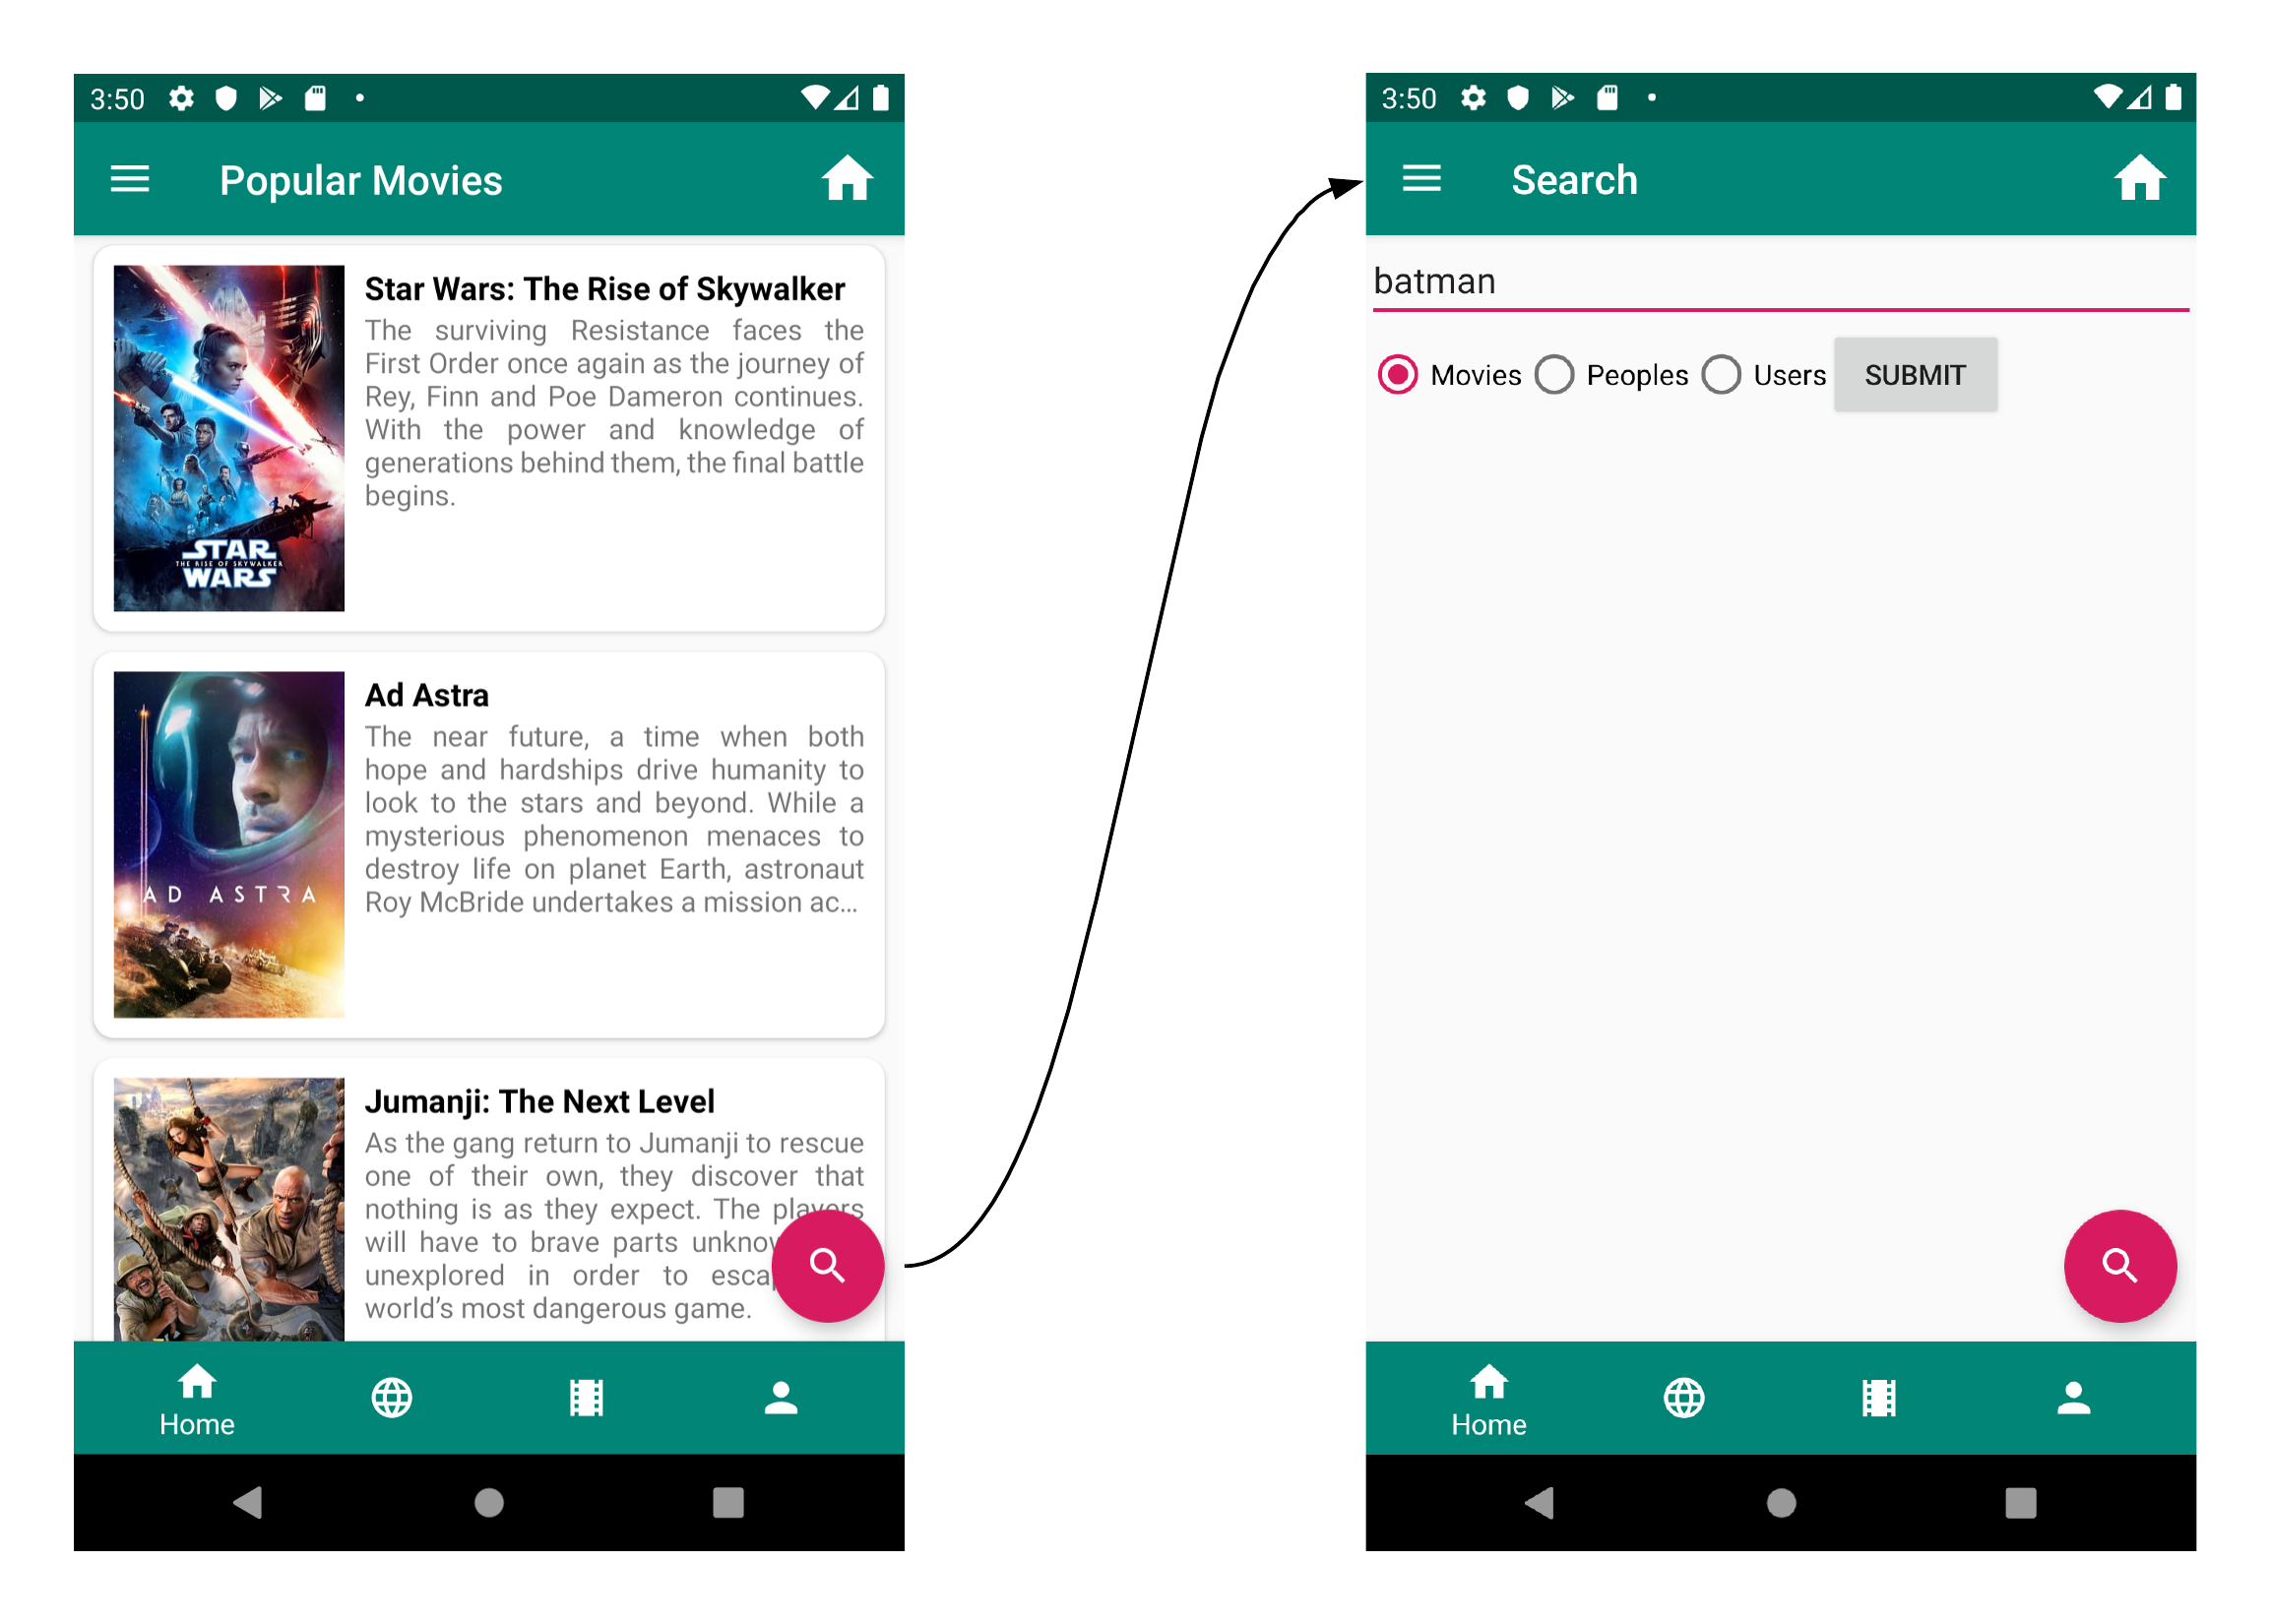
\includegraphics[width=0.8\textwidth]{img/screenshots/FAB.png}
    \end{center}
    \caption{FAB de l'application}
    \label{fab}
\end{figure}

\subsection{Generic adapter}\label{generic-adapter}
Dans le cadre de cette application, nous travaillons très fréquemment avec la \textit{recycler view} qui affiche une liste d'items, d'un même type pour toute la liste. Afin de ne pas devoir recréer une \textit{recycler view} par type d'items, nous avons choisi d'implémenter un adapteur générique permettant de réutiliser la même liste mais avec des items et layouts de type différents, comme illustré à la figure \ref{generic_adapter_img}.
\begin{figure}
    \begin{center}
        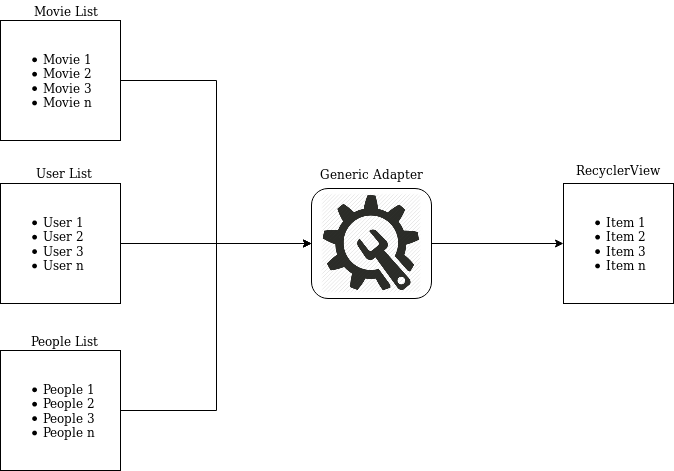
\includegraphics[width=0.8\textwidth]{img/schemas/Generic_Adapter.png}
    \end{center}
    \caption{Principes de l'adapteur générique}
    \label{generic_adapter_img}
\end{figure}